%------------------------------------------------------------------------------
% Author(s):
% Varaun Ramgoolie
%
% Copyright:
%  Copyright (C) 2020 Brad Bachu, Arjun Mohammed, Varaun Ramgoolie, Nicholas Sammy
%
%  This file is part of Applied-Mathematics-Unit2 and is distributed under the
%  terms of the MIT License. See the LICENSE file for details.
%
%  Description:
%     Year: 2011
%     Module: 3
%     Question: 6
%------------------------------------------------------------------------------

%------------------------------------------------------------------------------
% 6 a
%------------------------------------------------------------------------------

\begin{subquestions}
	
\subquestion
We are given the motion of an electric train.

\begin{subsubquestions}
	
\subsubquestion

\textbf{\textit{Sketch and Translate:}} \\ \\
\rfig{2011:q6:VTGraph} shows the velocity-time graph of the train.
\begin{figure}[H]
	\begin{center}
		\includegraphics{../2011/figures/2011q6-v-t-graph}
		\caption{\label{2011:q6:VTGraph} Velocity-time graph of the train}
	\end{center}
\end{figure}
As the train starts at rest, its initial velocity, $u$, at $t=0$ is 0.
\{Also will add a disp-time graph of the motion. \}

%------------------------------------------------------------------------------

\subsubquestion

\textbf{\textit{Simplify and Diagram:}} \\ \\ 
We can use \rfig{2011:q6:VTGraph} to find the initial acceleration of the train. We know that the area under a velocity-time graph gives the train's displacement. We also know that the gradient of a velocity-time graph gives the acceleration of the train. Therefore, we can use the information given to formulate simultaneous equations and find the acceleration of  the train.
Let us define:
\begin{itemize}
	\item $u$ is the initial velocity of the train at a point in time,
	\item $v$ is the final velocity of the train after a period of time,
	\item $s$ is the displacement of the train after a period of time,
	\item $a$ is the acceleration of the train. 
\end{itemize}



\textbf{\textit{Represent Mathematically:}} \\ \\
Firstly, we will represent the entire area, $A$, under the graph as,
\begin{align}
	A & = \text{Area of trapezium} \nn \\
	  & = \frac{6 + (t_2-t_1)}{2}\times V_{max} \,. \label{2011:q6:AEqn1}
\end{align}   
	
We will represent the area under the graph from $t_1$ to $t_2$, $A_1$, as,
\begin{align}
	A_1 & = \text{Area of rectangle} \nn \\
	& = (t_2-t_1)\times V_{max} \,. \label{2011:q6:AEqn2}
\end{align}  
	
By using these equations, we can find the initial acceleration of the train by using,
\begin{equation}
	v^2 = u^2 + 2as  \label{2011:q6:AEqn3} \,. 
\end{equation} 



\textbf{\textit{Solve and Evaluate:}} \\ \\
By substituting $A_1=1.5$km into \req{2011:q6:AEqn2}, we get that,
\begin{align}
	1.5 & = (t_2-t_1)\times V_{max} \nn \\
	\implies (t_2-t_1) & = \frac{1.5}{V_{max}} \,.
\end{align}

As the total journey was 2.3km, we substitute $A=2.3$km and $(t_2-t_1) = \frac{1.5}{V_{max}}$ into \req{2011:q6:AEqn1} to find,
\begin{align}
	2.3 & = \frac{6 + (t_2-t_1)}{2}\times V_{max} \nn \\
		& = 3V_{max} + \frac{(t_2-t_1)}{2}V_{max} \nn \\
		& = 3V_{max} + \frac{1.5}{2V_{max}}V_{max} \nn \\
		\implies V_{max} & = \frac{2.3-0.75}{3} = \frac{31}{60} \text{km/min} \nn \\
		               & = 31\text{km/hr} \,.
\end{align}

Finally, considering the motion between $t=0$ and $t_1$ with $v=31$km/hr, $u=0$km/hr and $s=0.5$km, we use \req{2011:q6:AEqn3} to get that,
\begin{align}
	31^2 & = 0^2 + 2(a)(0.5) \nn \\
	a & = \frac{31^2-0^2}{2(0.5)} \nn \\
	  & = 961 ~km/hr^2 \,.
\end{align}

\end{subsubquestions}	
	
%------------------------------------------------------------------------------
% 6 b
%------------------------------------------------------------------------------
	
\subquestion

\begin{subsubquestions}

\subsubquestion

\textbf{\textit{Sketch and Translate:}} \\ \\
We are given a block which moves up along fixed guides. As we are given the force which moves the block, we should begin thinking about how the force is related to the work done.
\begin{figure}[H]
	\begin{center}
		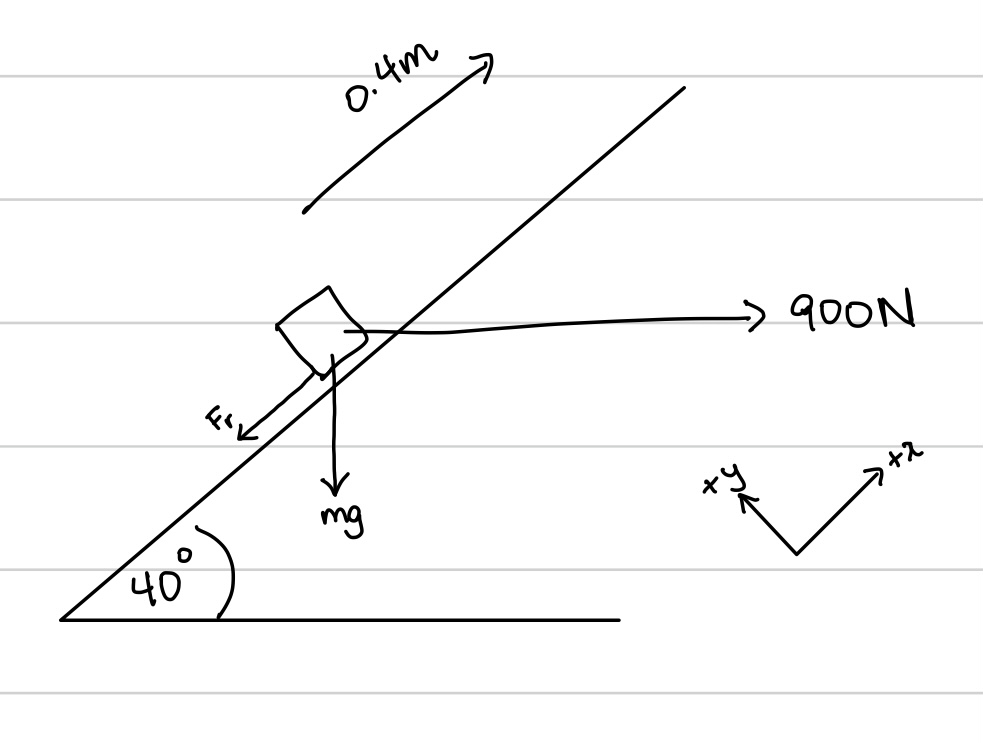
\includegraphics[scale=0.25]{../2011/figures/2011q6-1}
		\caption{\label{2011:q6:Sketch2} Block moving up the guide.}
	\end{center}
\end{figure}
	
	
	
	
\textbf{\textit{Simplify and Diagram:}} \\ \\
\begin{figure}[H]
	\begin{center}
		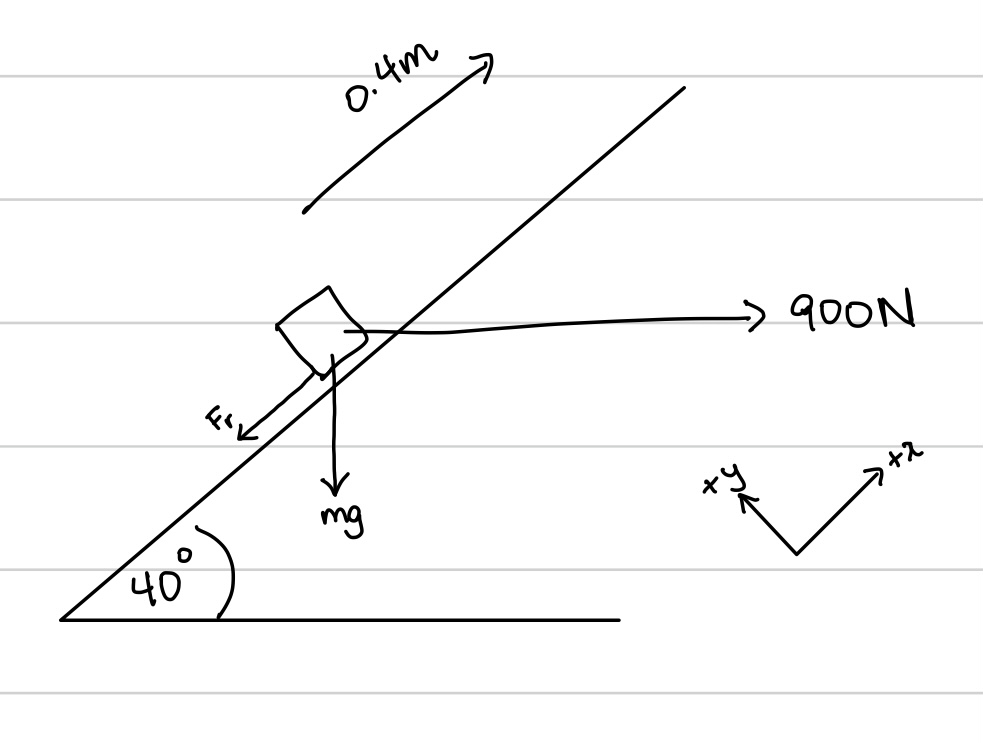
\includegraphics[scale=0.25]{../2011/figures/2011q6-1}
		\caption{\label{2011:q6:Diagram2} Block moving up the guide.}
	\end{center}
\end{figure}
By using the information given and our definition for Work, we can substitute our values and solve for the work done.




\textbf{\textit{Represent Mathematically:}} \\ \\
By definition, we know that,
\begin{equation}
	\text{Work Done} = \text{Force} \times \text{Distance traveled in the direction of the force} \,.
\end{equation}

We must also find the component of the 900N force in the direction of the slope. By resolving, we get that,
\begin{align}
	\vec{900} & = |900|\cos(40) \xhat -|900|\sin(40) \yhat \,.
\end{align}




\textbf{\textit{Solve and Evaluate:}} \\ \\
As the block has moved 0.4m in the $x$ direction, we must consider the $x$ component of the 900N force as follows,
\begin{align}
	\text{Work Done} & = \text{Force} \times \text{Distance traveled in the direction of the force} \nn \\
	                 & = |900|\cos(40) \times 0.4 \nn \\
	                 & = 275.8 J \,.
\end{align}

%------------------------------------------------------------------------------

\subsubquestion

\textbf{\textit{Simplify and Diagram:}} \\ \\
\begin{figure}[H]
	\begin{center}
		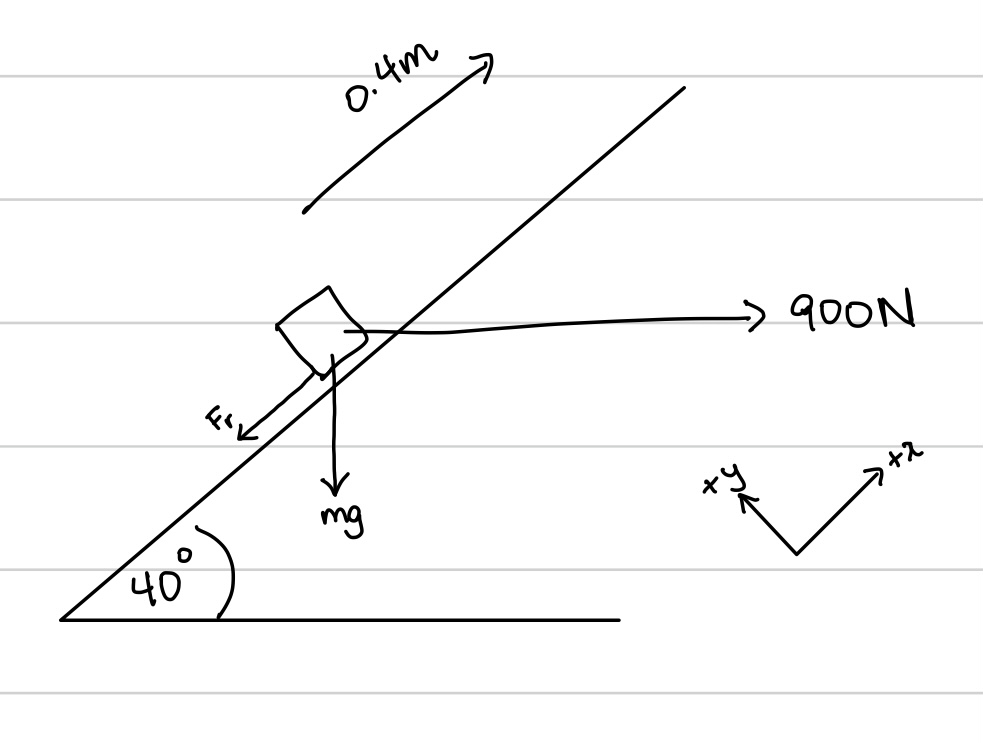
\includegraphics[scale=0.25]{../2011/figures/2011q6-1}
		\caption{\label{2011:q6:Diagram3} Block moving up the guide, with all the forces acting on it.}
	\end{center}
\end{figure}

Let us define the following as,
\begin{itemize}
	\item $\vec{W}$ which is the weight if the block,
	\item $\vec{R}$ which is the normal reaction force,
	\item $F_f$ which is the frictional force,
	\item $F_{p}$ which is the 900N force which moves the block,
	\item $m$ which is the mass of the block, $m=70$.
\end{itemize}
We will assume that the body acts as a point particle and that there are no other forces acting on the body, We will also assume that the block is in equilibrium. We can consider Newton's Second Law and find the magnitude of the frictional force.




\textbf{\textit{Represent Mathematically:}} \\ \\
Let us first resolve all the forces as,
\begin{align}
	\vec{W} & = -|W|\sin(40)\xhat - |W|\cos(40)\yhat  \\ 
	\vec{R} & = |R|\yhat  \\ 
	\vec{F_f} & = -|F_f|\xhat  \\
	\vec{F_p} & = |F_p|\cos(40) \xhat -|F_p|\sin(40) \yhat \,.
\end{align}

Under our assumption that there is no net resultant force (and by extension, no net acceleration), we can consider Newton's Second Law in the $x$ direction as,
\begin{equation}
	\sum F_x = 0 \,. \label{2011:q6:Newt1}
\end{equation}




\textbf{\textit{Solve and Evaluate:}} \\ \\
By substituting our values into \req{2011:q6:Newt1}, we get that,
\begin{align}
	\sum F_x & = 0 \nn \\
	-|W|\sin(40)-|F_f|+|F_p|\cos(40) & = 0 \nn \\
	\implies |F_f| & = |F_p|\cos(40)-|W|\sin(40) \nn \\
	               & = 900\cos(40)-mg\sin(40) \nn \\
	               & = 900\cos(40)-(70)(10)\sin(40) \nn \\
	               & = 239.5N \,.
\end{align}

\end{subsubquestions}
	
	
	
	
\end{subquestions}





















